\section{Methodology}
\begin{figure*}[t]
\centering
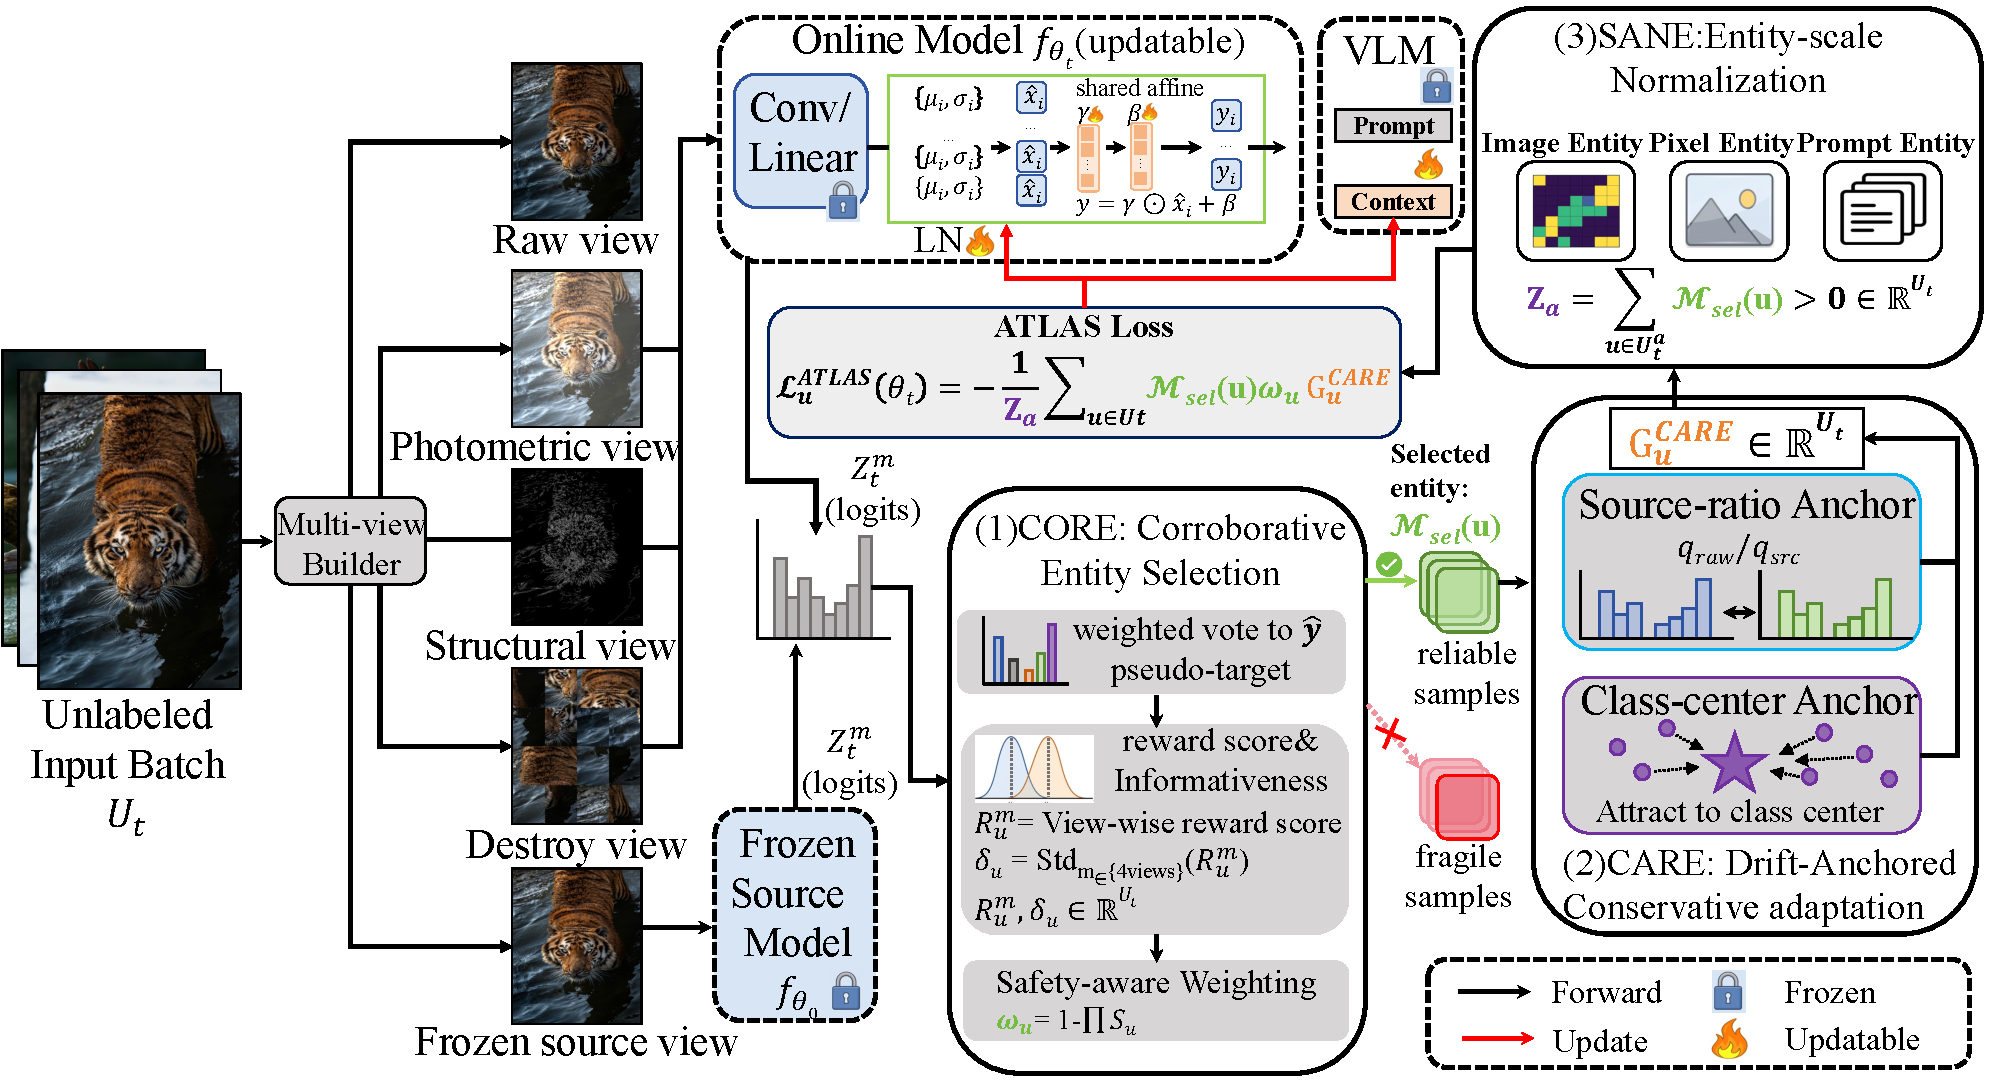
\includegraphics[width=1\linewidth]{figures/fig2-2.pdf}
\caption{Overview of the ATLAS framework. ATLAS builds multiple target views, selects safe and informative entities through CORE, constrains their updates with CARE, and normalizes the loss with SANE, updating only lightweight normalization or prompt parameters.}
\label{fig:atlas_pipeline}
\end{figure*}


\subsection{Problem setup}

Let $f(x;\theta)$ be a source model trained on a labeled source domain
$\mathcal{D}_s=\{(x_i,y_i)\}_{i=1}^{N}$ and deployed on an unlabeled target
stream $\mathcal{D}_t=\{x_t\}_{t=1}^{T}$. Fully test-time adaptation updates
the model online from target observations only~\citep{wang2021tent,niu2022eata}.
The classical entropy-minimization objective is
\begin{equation}
\mathcal{L}_{\mathrm{ent}}(x_t;\theta)
=
-\sum_{c=1}^{C}
p_{\theta}(y=c\mid x_t)\log p_{\theta}(y=c\mid x_t),
\qquad
p_{\theta}(\cdot\mid x_t)=\mathrm{softmax}(f(x_t;\theta)).
\label{eq:tent}
\end{equation}
Although this objective encourages confident predictions, it does not ask
whether confidence is corroborated, whether the update is anchored, or whether
losses are comparable across entity granularities.

This entity-centric view is close to slot-centric test-time adaptation, which studies decomposed object-centric representations rather than only whole-image predictions~\citep{prabhudesai2023test}.

ATLAS organizes its task-specific instantiations around primitive prediction entities. Let $B$ be the
target batch size, $\Omega_i$ the spatial lattice of image $i$, and $V$ the
number of prompt views. The entity set is
\begin{equation}
\begin{aligned}
\mathcal{U}_t^{\mathrm{img}}
&=\{\,i\,\}_{i=1}^{B},\\
\mathcal{U}_t^{\mathrm{pix}}
&=\{\,(i,s): i=1,\ldots,B,\; s\in\Omega_i\,\},\\
\mathcal{U}_t^{\mathrm{prm}}
&=\{\,(i,v): i=1,\ldots,B,\; v=1,\ldots,V\,\}.
\end{aligned}
\label{eq:entity_sets}
\end{equation}
Thus $u=i$ denotes an image-level prediction vector, $u=(i,s)$ a pixel-level
vector, and $u=(i,v)$ a prompt-view vector. The notation $\mathcal{U}_t^a$
denotes the active set, where
$a\in\{\mathrm{img},\mathrm{pix},\mathrm{prm}\}$.

For each entity, \method{} compares a frozen-source prediction, the current raw
prediction, a photometric view, a structural view, and a destroy view. Let
$z_u^m\in\mathbb{R}^{C}$ denote the pre-softmax logit vector for entity $u$
under view $m$, and let $p_u^m$ denote the corresponding class-probability
vector:
\begin{equation}
\mathcal{M}_{\mathrm{sup}}
=
\{\mathrm{src},\mathrm{raw},\mathrm{pho},\mathrm{str}\},
\qquad
\mathcal{M}_{\mathrm{all}}
=
\mathcal{M}_{\mathrm{sup}}\cup\{\mathrm{des}\},
\qquad
p_u^m=\mathrm{softmax}(z_u^m).
\label{eq:view_prob}
\end{equation}
The destroy view deliberately disrupts structure, e.g., by patch shuffling, to expose fragile confidence.


\subsection{Corroborative Entity Selection}

\core{} selects reliable entities from the view probabilities
$\{p_u^m\}_{m\in\mathcal{M}_{\mathrm{all}}}$. It first forms a pseudo-target by weighted voting:
\begin{equation}
\hat y_u
=
\arg\max_{c\in\mathcal{Y}}
\sum_{m\in\mathcal{M}_{\mathrm{sup}}}
\alpha_u^m
\mathbf{1}\!\left[
\arg\max_{j\in\mathcal{Y}}p_u^m(j)=c
\right],
\qquad
\alpha_u^m=\max_{c\in\mathcal{Y}}p_u^m(c)+\eta_m ,
\label{eq:vote}
\end{equation}
where $\eta_{\mathrm{src}}>0$ is a small source prior and $\eta_m=0$ for all $m\neq \mathrm{src}$.
The target-class probability is
\begin{equation}
q_u^m=p_u^m(\hat y_u),
\qquad
m\in\mathcal{M}_{\mathrm{all}}.
\label{eq:target_prob}
\end{equation}

Let
\begin{equation}
\bar H_u^m
=
-\frac{1}{\log C}
\sum_{c=1}^{C}p_u^m(c)\log p_u^m(c)
\label{eq:normalized_entropy}
\end{equation}
denote normalized entropy. We aggregate the four normalized evidence terms by
an equal mean, avoiding learned or benchmark-selected reward coefficients:
\begin{equation}
\begin{aligned}
R_u^m
=\frac{1}{4}\Big(&q_u^m+(1-\bar H_u^m)
+
\mathbf{1}\!\left[
\arg\max_c p_u^m(c)=\arg\max_c p_u^{\mathrm{src}}(c)
\right]
+
\mathbf{1}\!\left[
\arg\max_c p_u^m(c)=\hat y_u
\right]\Big).
\end{aligned}
\label{eq:reward}
\end{equation}
Its dispersion
\begin{equation}
\delta_u
=
\mathrm{Std}_{m\in\{\mathrm{raw},\mathrm{pho},\mathrm{str},\mathrm{des}\}}
(R_u^m)
\label{eq:dispersion}
\end{equation}
measures whether the views provide differential evidence.

The safety score combines entropy, source disagreement, view inconsistency, and insufficient destroy-view sensitivity:
\begin{equation}
s_u
=
\lambda_e\bar H_u^{\mathrm{raw}}
+\lambda_a\Delta_u^{\mathrm{anchor}}
+\lambda_v\Delta_u^{\mathrm{view}}
+\lambda_d[\rho_d-\Delta_u^{\mathrm{des}}]_+,
\label{eq:safety_score}
\end{equation}
with
\begin{equation}
\begin{aligned}
\Delta_u^{\mathrm{anchor}}
&=
\mathbf{1}\!\left[
\arg\max_c p_u^{\mathrm{raw}}(c)
\ne
\arg\max_c p_u^{\mathrm{src}}(c)
\right],\\
\Delta_u^{\mathrm{view}}
&=
1-\frac{1}{2}
\sum_{m\in\{\mathrm{pho},\mathrm{str}\}}
\mathbf{1}\!\left[
\arg\max_c p_u^m(c)
=
\arg\max_c p_u^{\mathrm{raw}}(c)
\right],\\
\Delta_u^{\mathrm{des}}
&=
[q_u^{\mathrm{raw}}-q_u^{\mathrm{des}}]_+ .
\end{aligned}
\label{eq:safety_terms}
\end{equation}
Here $\rho_d>0$ is the minimum destroy-view confidence drop required before an entity is treated as structurally supported.
The soft safety weight is
\begin{equation}
\omega_u
=
1-\Pi(s_u;m_{\mathrm{safe}},m_{\mathrm{hard}}),
\qquad
\Pi(s;m_{\mathrm{safe}},m_{\mathrm{hard}})
=
\begin{cases}
0, & s\le m_{\mathrm{safe}},\\[2pt]
\dfrac{s-m_{\mathrm{safe}}}{m_{\mathrm{hard}}-m_{\mathrm{safe}}},
& m_{\mathrm{safe}}<s<m_{\mathrm{hard}},\\[8pt]
1, & s\ge m_{\mathrm{hard}}.
\end{cases}
\label{eq:safe}
\end{equation}
For the Core variant, the normalized evidence terms define a reliability score
$e_u$ (their available-term mean), and the final selection mask is
\begin{equation}
\mathcal{M}_{\mathrm{sel}}(u)
=
\mathbf{1}\!\left[e_u\ge Q_q(\{e_v:v\in\mathcal U_t\})\right],
\label{eq:selected}
\end{equation}
where $Q_q$ is computed only from the current unlabeled adaptation entities and
$q=0.5$ throughout. Thus the Core gate transfers by score order rather than an
absolute entropy, PLPD, dispersion, or safety threshold. Full retains the
branch refinements audited in the supplement and is reported separately.

\subsection{Drift-Anchored Conservative Adaptation}

\care{} anchors the update of selected entities. When source support is reliable, it uses the raw-view advantage
\begin{equation}
A_u
=
\frac{
R_u^{\mathrm{raw}}
-
\frac{1}{4}
\sum_{m\in\{\mathrm{raw},\mathrm{pho},\mathrm{str},\mathrm{des}\}}R_u^m
}
{\delta_u+\varepsilon}
\label{eq:advantage}
\end{equation}
and the entity-level source-relative ratio
\begin{equation}
r_u
=
\frac{q_u^{\mathrm{raw}}+\varepsilon}
{q_u^{\mathrm{src}}+\varepsilon}.
\label{eq:ratio}
\end{equation}
The conservative clipped surrogate is
\begin{equation}
\phi(r_u,A_u)
=
\min\!\left(
r_uA_u,\,
\operatorname{clip}(r_u,1-\epsilon_{\mathrm{low}},1+\epsilon_{\mathrm{high}})A_u
\right).
\label{eq:clip}
\end{equation}
The signed advantage and two-sided PPO surrogate prevent improvement beyond the
upper clip for $A_u>0$ and prevent deterioration beyond the lower clip for
$A_u<0$. Eq.~\ref{eq:atlas_loss} minimizes its negative normalized form.

When class structure is more reliable than direct source matching, \care{} uses a class-centered anchor. For pseudo-class $\hat y_u$ with online
center $c_{\hat y_u}^t\in\mathbb{R}^{C}$,
\begin{equation}
\ell_u^{\mathrm{center}}
=
\frac{(p_u^{\mathrm{raw}}-\operatorname{stopgrad}(c_{\hat y_u}^{t}))^\top
z_u^{\mathrm{raw}}}{g_u},
\quad
g_u=\left\|\bigl(z_u^{\mathrm{raw}}+T_u+1\bigr)\odot
p_u^{\mathrm{raw}}\right\|_1,
\quad
T_u=-\sum_c p_u^{\mathrm{raw}}(c)z_u^{\mathrm{raw}}(c).
\label{eq:centered}
\end{equation}
The stopped-gradient center is the conservative reference. The scale $g_u$ is
also detached; a finite-difference test verifies that a descent step reduces
$D_{\mathrm{KL}}(c_{\hat y_u}^{t}\|p_u^{\mathrm{raw}})$. The entity-level \care{} support is
\begin{equation}
G_{\mathrm{u}}^{CARE}
=
\begin{cases}
\phi(r_u,A_u),
& \text{source-relative anchor},\\[2pt]
-\ell_u^{\mathrm{center}},
& \text{class-centered anchor},\\[2pt]
0,
& \text{otherwise}.
\end{cases}
\label{eq:anc_entity}
\end{equation}
Equivalently, the per-entity loss is $\ell_{\mathrm{u}}^{CARE}=-G_{\mathrm{u}}^{CARE}$ before entity-scale normalization.

\subsection{Entity-Scale Normalization}

\sane{} normalizes by the number of selected primitive prediction entities.
% The uppercase symbol $Z_a$ denotes this entity-scale normalizer, which
% is distinct from the lowercase logits $z_u^m$ defined above.
For the three scenarios,
\begin{equation}
Z_{\mathrm{img}}
=
\sum_{i=1}^{B}\mathcal{M}_{\mathrm{sel}}(i),
\qquad
Z_{\mathrm{pix}}
=
\sum_{i=1}^{B}\sum_{s\in\Omega_i}\mathcal{M}_{\mathrm{sel}}(i,s),
\qquad
Z_{\mathrm{prm}}
=
\sum_{i=1}^{B}\sum_{v=1}^{V}\mathcal{M}_{\mathrm{sel}}(i,v).
\label{eq:sane_three_cases}
\end{equation}
% \begin{equation}
% \begin{aligned}
% Z_{\mathrm{img}}
% &=
% \sum_{i=1}^{B}
% \mathcal{M}_{\mathrm{sel}}(i),\\
% Z_{\mathrm{pix}}
% &=
% \sum_{i=1}^{B}
% \sum_{s\in\Omega_i}
% \mathcal{M}_{\mathrm{sel}}(i,s),\\
% Z_{\mathrm{prm}}
% &=
% \sum_{i=1}^{B}
% \sum_{v=1}^{V}
% \mathcal{M}_{\mathrm{sel}}(i,v).
% \end{aligned}
% \label{eq:sane_three_cases}
% \end{equation}
Equivalently,
\begin{equation}
Z_a
=
\sum_{u\in\mathcal{U}_t^a}
\mathcal{M}_{\mathrm{sel}}(u),
\qquad
a\in\{\mathrm{img},\mathrm{pix},\mathrm{prm}\}.
\label{eq:sane_unified}
\end{equation}

If $Z_a=0$, the adaptation step is skipped. Evidence weights in the numerator
are detached, while the denominator is the integer selected-entity count rather
than weighted mass or total output size. In the denominator, ATLAS uses a small
constant $\varepsilon_Z>0$ for numerical stability.

\subsection{The \atlasloss{}}

\core{}, \care{}, and \sane{} yield the final objective
\begin{equation}
\mathcal{L}_{\text{\textsc{ATLAS}}}^{a}(\theta_t)
=
-\frac{1}{Z_a+\varepsilon_Z}
\sum_{u\in\mathcal{U}_t^a}
\underbrace{
\mathcal{M}_{\mathrm{sel}}(u)\omega_u
}_{\text{\core{} selection}}
\underbrace{
G_{\mathrm{u}}^{CARE}
}_{\text{\care{} anchoring}},
\qquad
a\in\{\mathrm{img},\mathrm{pix},\mathrm{prm}\}.
\label{eq:atlas_loss}
\end{equation}
Thus \core{} selects reliable entities, \care{} anchors their update direction, and \sane{} makes the loss comparable across image-, pixel-, and prompt-view adaptation. Appendix~\ref{app:atlas_executable} starts with a compact principle-versus-instantiation table and then records the online update used in the artifact, including the scenario-specific gate $\gamma_u$, the exposed paper-level hyperparameters, the EMA class-center update, and the branch-level choice between the two CARE anchors.

% \subsection{Scenario instantiations}

% \paragraph{Classification.}
% The active set is $\mathcal{U}_t^{\mathrm{img}}$, where each entity $u=i$ is one
% image-level prediction vector. The normalizer is $Z_{\mathrm{img}}$.

% \paragraph{Segmentation.}
% The active set is $\mathcal{U}_t^{\mathrm{pix}}$, where each entity $u=(i,s)$ is
% one pixel-level prediction vector at location $s$. The normalizer is
% $Z_{\mathrm{pix}}$.

% \paragraph{Vision-language adaptation.}
% The active set is $\mathcal{U}_t^{\mathrm{prm}}$, where each entity $u=(i,v)$ is
% one prompt-view prediction vector. The normalizer is $Z_{\mathrm{prm}}$.
